\begin{frame}[allowframebreaks]{Vector Quantized - Variational Autoencoders}
\begin{figure}
        \centering
        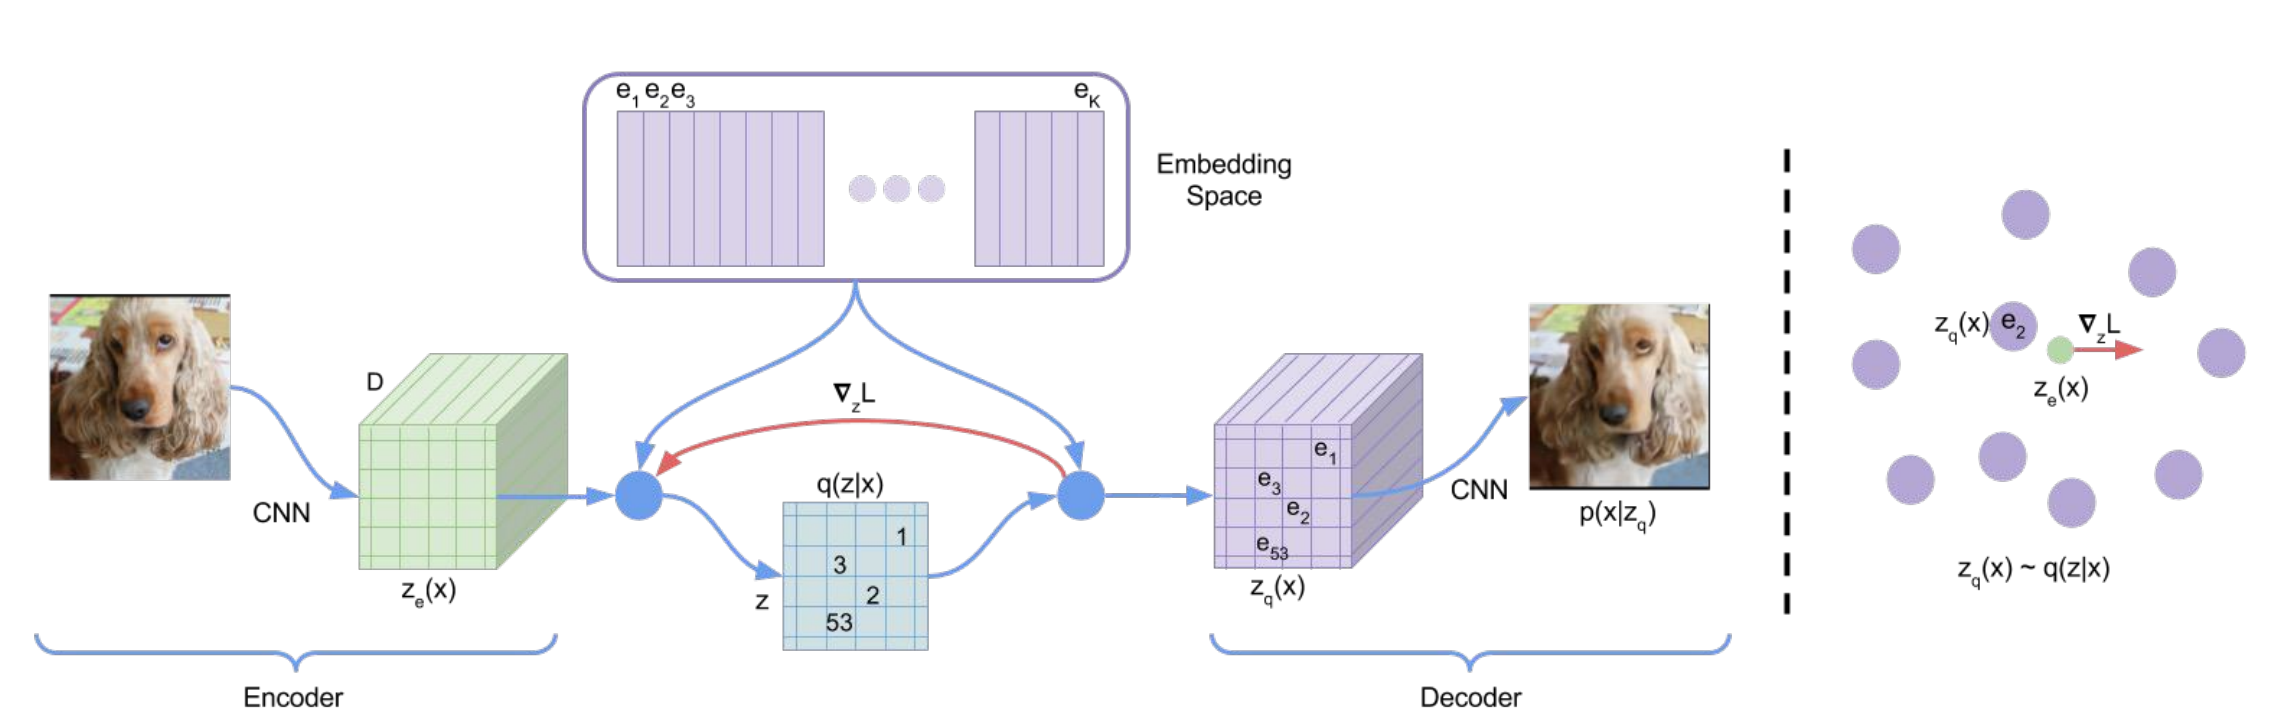
\includegraphics[height=0.9\textheight, width=\textwidth, keepaspectratio]{images/vae/vqvae.PNG}
\end{figure}
\end{frame}

\begin{frame}[allowframebreaks]{Vector Quantized - Variational Autoencoders}

\begin{itemize}
    \item A latent embedding space $e \in \mathbb{R}^{K \times D}$ where $K$ is the size of the discrete latent space (K-way categorical distribution)
    \item  Encoder output $z_e(x)$ is mapped to discrete latent code z by a nearest neighbour look-up using the shared embedding space $e$
    \item The posterior categorical distribution $q(z|x)$ probabilities are defined as one-hot as:
    \[ q(z = k|x) = \begin{cases} 
          1 & \text{for } k = argmin_j ||z_e(x) - e_j||_2 \\
          0 & \text{otherwise}
       \end{cases}
    \]
\end{itemize}
\end{frame}

\begin{frame}[allowframebreaks]{Vector Quantized - Variational Autoencoders}
\begin{itemize}
    \item  This model can be seen as a VAE in which the proposal distribution $q(z = k|x)$ is deterministic.
    \item The representation $z_e(x)$ is passed through the discretization bottleneck followed by mapping onto the nearest element of embedding $e$\\
    % \vspace{-1cm}
    $$z_q(x) = e_k, \hspace{1cm} \text{where} \hspace{0.5cm} k = argmin_j ||z_e(x) - e_j||_2$$
    % \vspace{-2cm}
    $$L = log \: p(x|z_q(x)) + ||sg[z_e(x)] - e||^2_2 + \beta||z_e(x) - sg[e]||_2^2$$
    % \vspace{-10pt}
    sg stands for the \textbf{stopgradient} operator that is defined as identity at forward computation time and has zero partial derivatives, thus effectively constraining its operand to be a non-updated constant. 
    \item The embedding space is learned via Vector Quantization (VQ), whose objective uses the $l_2$ error to move the embedding vectors $e_i$ towards the encoder outputs $z_e(x)$
    
\end{itemize}
\end{frame}

\begin{frame}{VQ-VAE}
    \begin{columns}
\begin{column}{0.4\textwidth}
   \begin{itemize}
       \item For speech, image and videos one can respectively extract a 1D, 2D and 3D latent feature spaces
       \item  32 x 32 latents for ImageNet, or 8 x 8 x 10 for CIFAR10
       \item 512-dimensional latents for VCTK and LibriSpeech
   \end{itemize}
\end{column}
\begin{column}{0.6\textwidth}  %%<--- here
    \begin{center}
     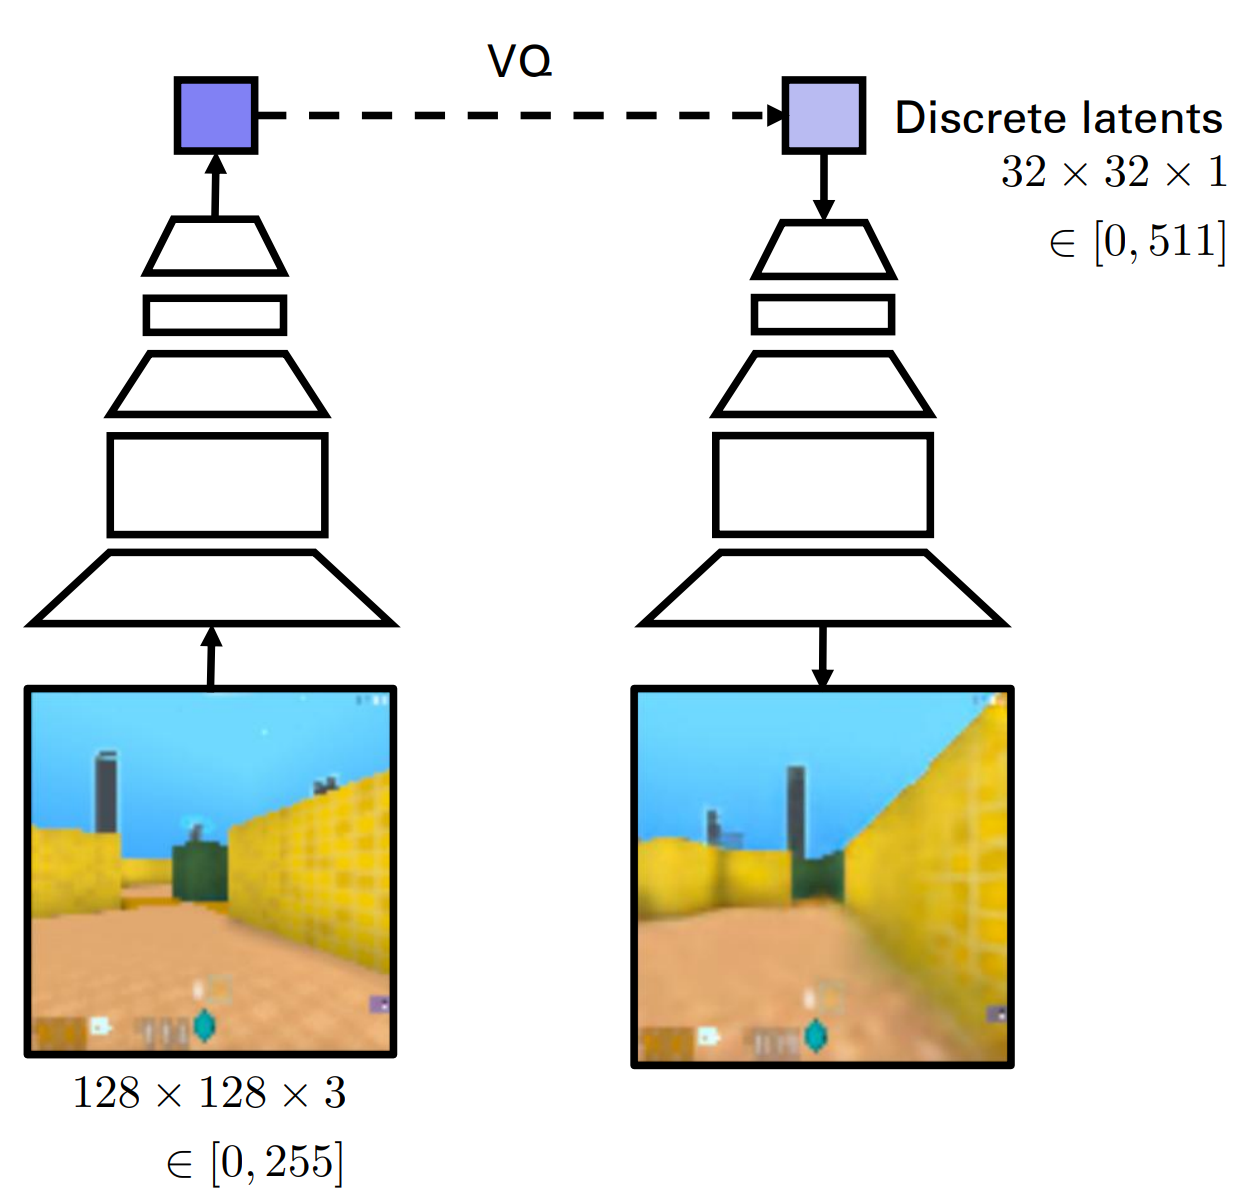
\includegraphics[height=0.9\textheight, width=\textwidth, keepaspectratio]{images/vae/vqvae_b.PNG}
     \end{center}
\end{column}
\end{columns}
\end{frame}

\begin{frame}[allowframebreaks]{VQ-VAE ImageNet Reconstruction}
\begin{figure}
        \centering
        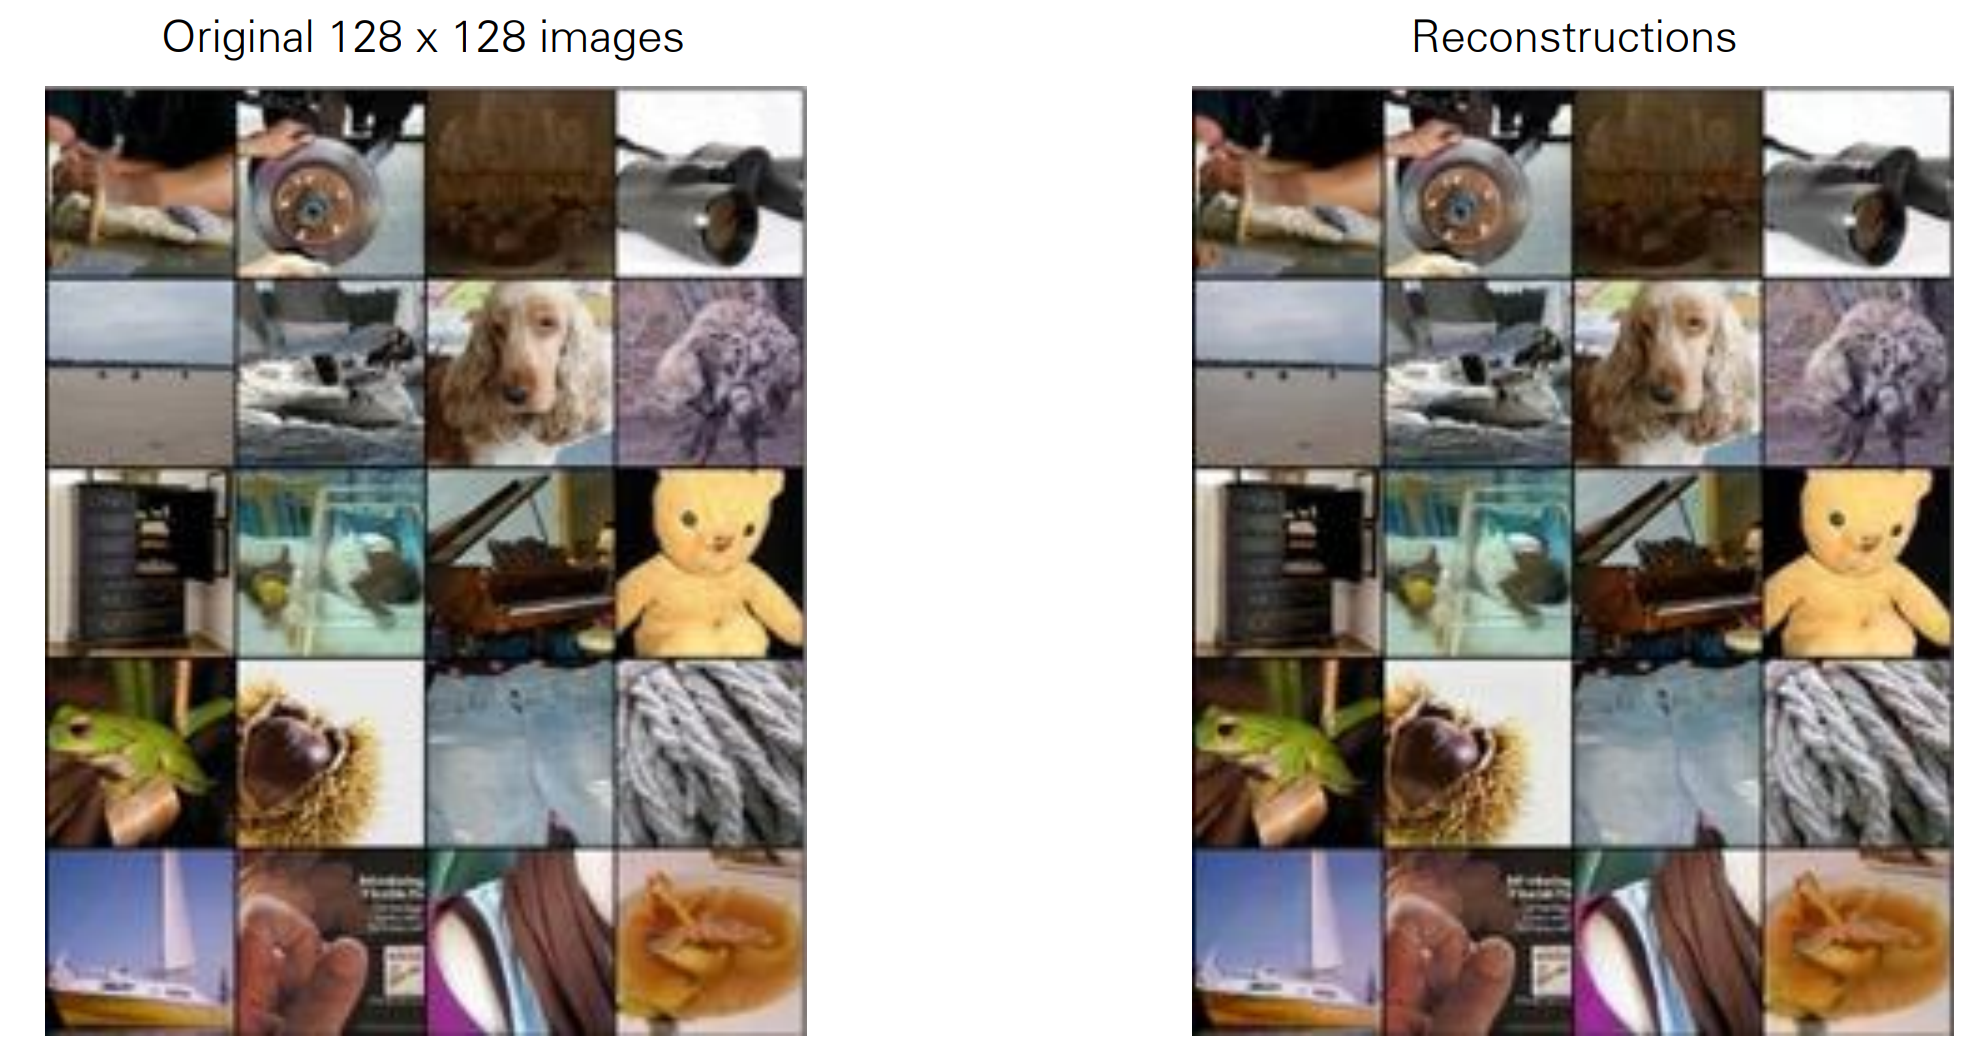
\includegraphics[height=0.9\textheight, width=\textwidth, keepaspectratio]{images/vae/vq_vae_reconstructions.PNG}
\end{figure}
\end{frame}

\begin{frame}[allowframebreaks]{VQ-VAE Sampling}
\begin{figure}
        \centering
        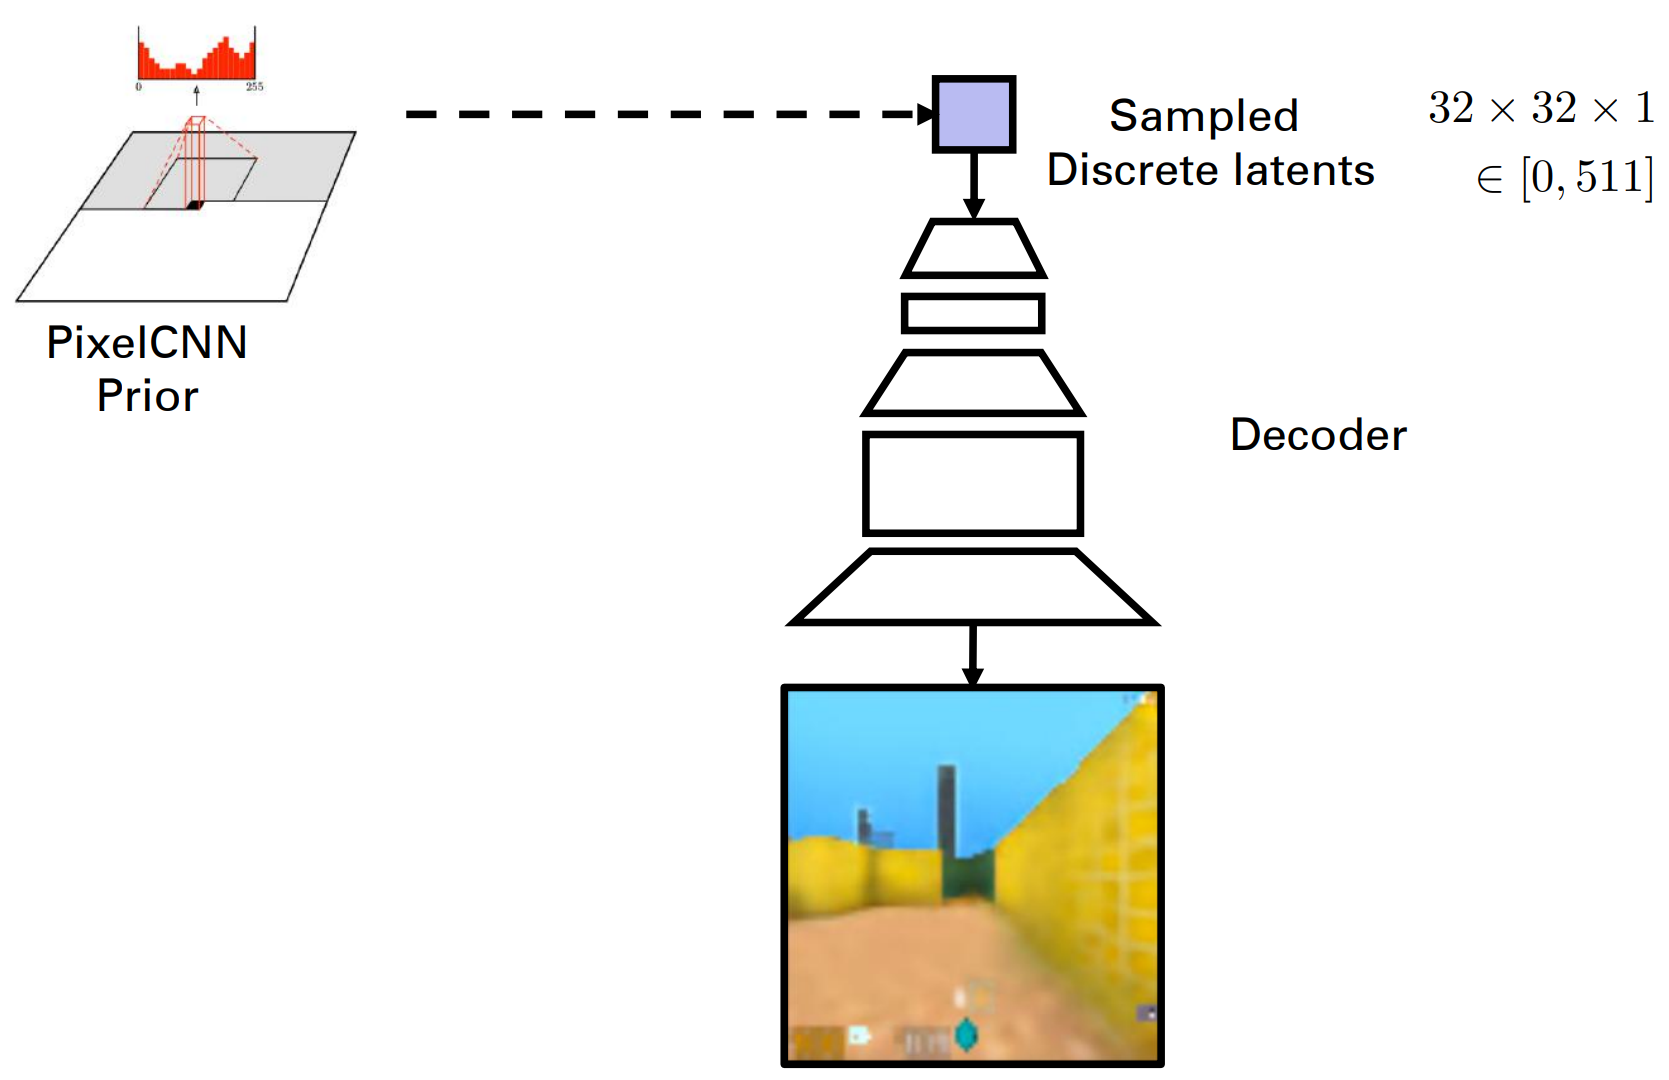
\includegraphics[height=0.9\textheight, width=\textwidth, keepaspectratio]{images/vae/vq_vae_sampling.PNG}
\end{figure}
\end{frame}

\begin{frame}[allowframebreaks]{VQ-VAE ImageNet Samples}
\begin{figure}
        \centering
        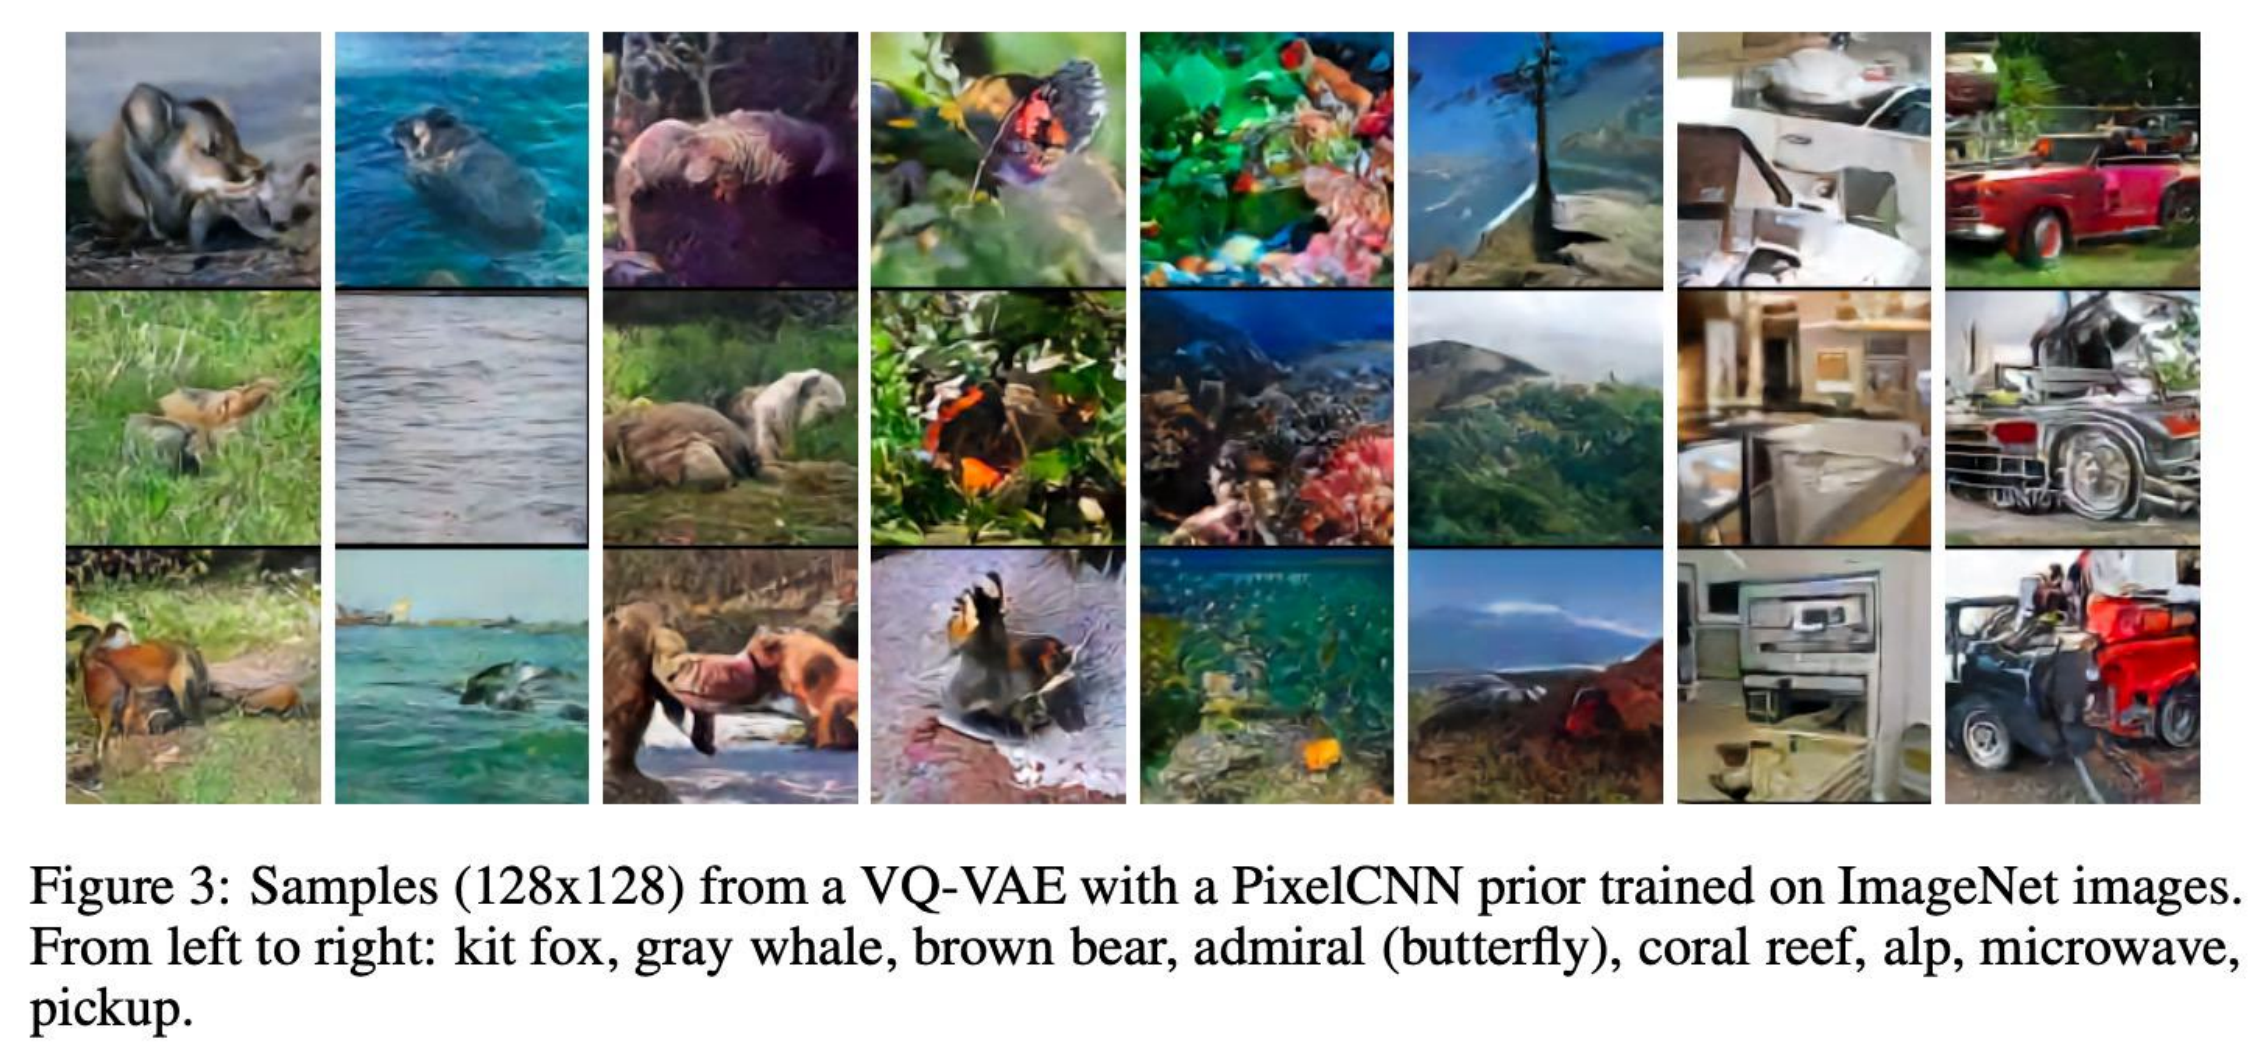
\includegraphics[height=0.9\textheight, width=\textwidth, keepaspectratio]{images/vae/vq_vae_samples.PNG}
\end{figure}
\end{frame}


\begin{frame}[allowframebreaks]{VQ-VAE Voice Style Transfer}
\begin{figure}
        \centering
        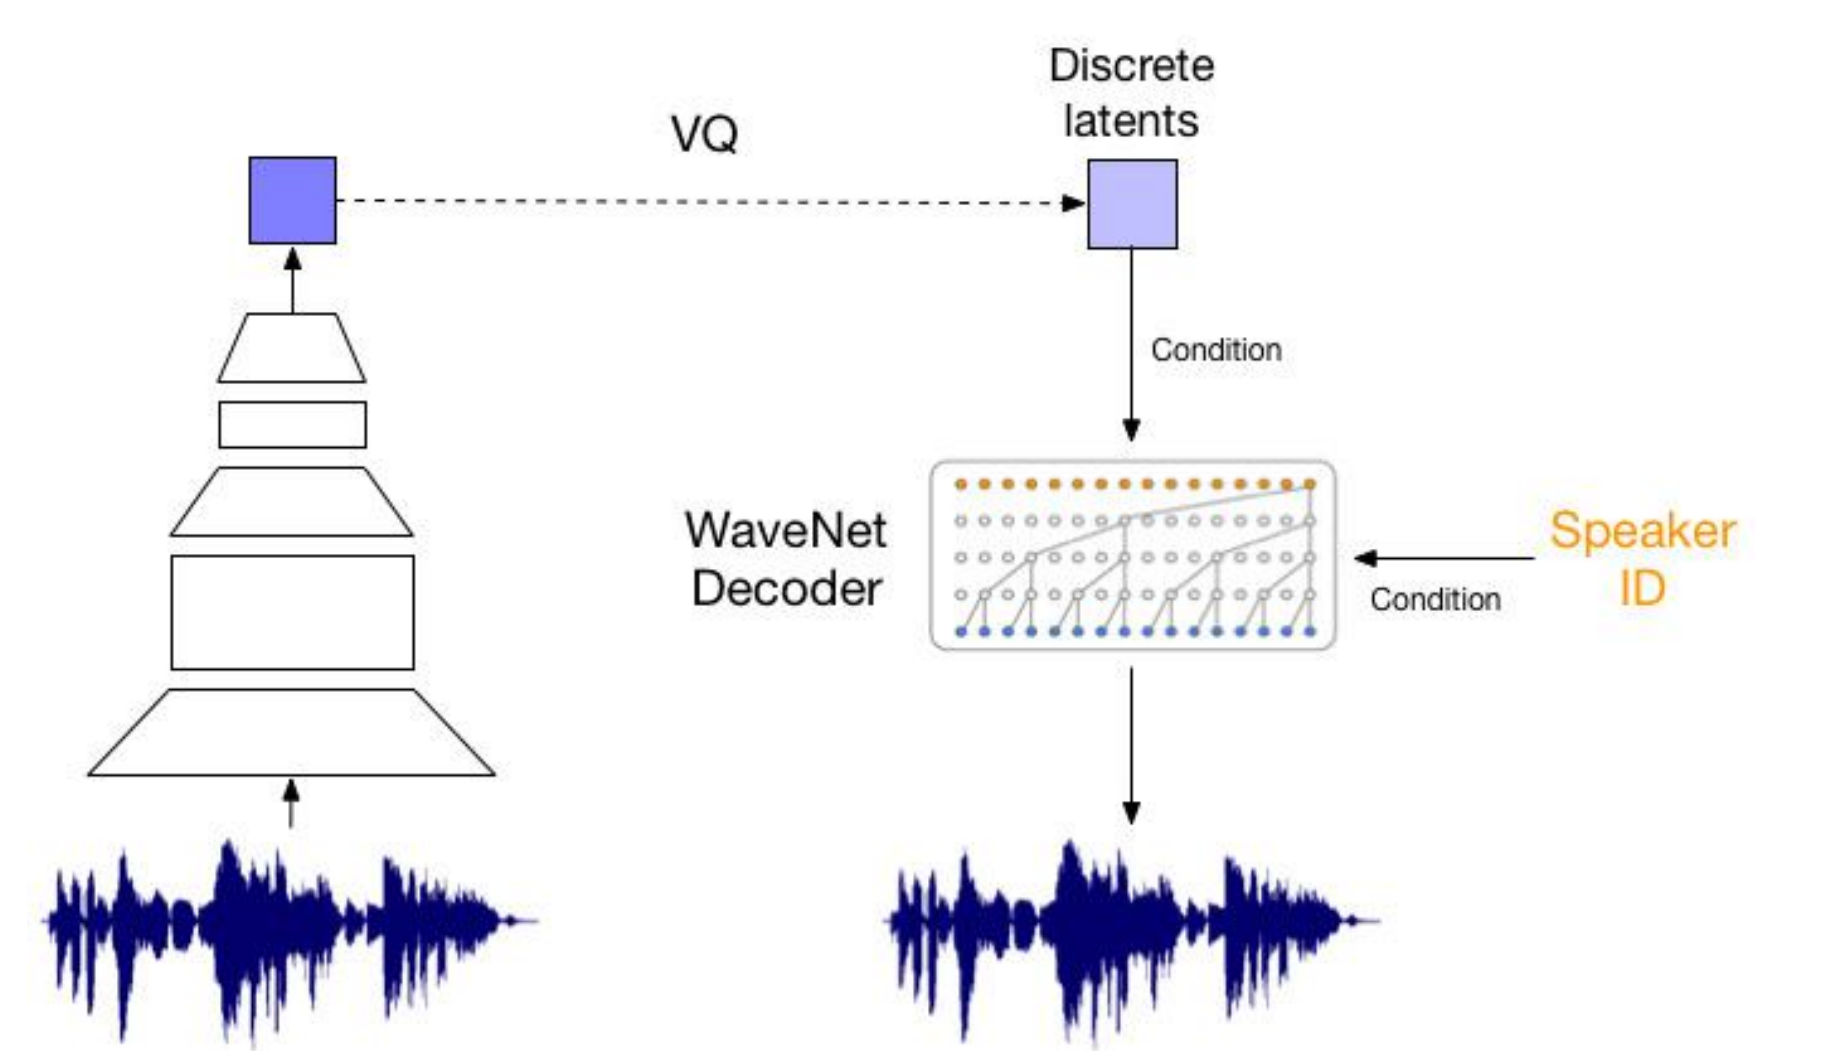
\includegraphics[height=0.9\textheight, width=\textwidth, keepaspectratio]{images/vae/vq_vae_voice.PNG}
\end{figure}
\end{frame}

\begin{frame}{VQ-VAE 2}
    \begin{columns}
\begin{column}{0.3\textwidth}
   \begin{itemize}
       \item The input 256×256 image is compressed to quantized latent maps of size 64×64 and 32×32
       \item The decoder reconstructs the image from the two latent maps.
   \end{itemize}
\end{column}
\begin{column}{0.7\textwidth}  %%<--- here
    \begin{center}
     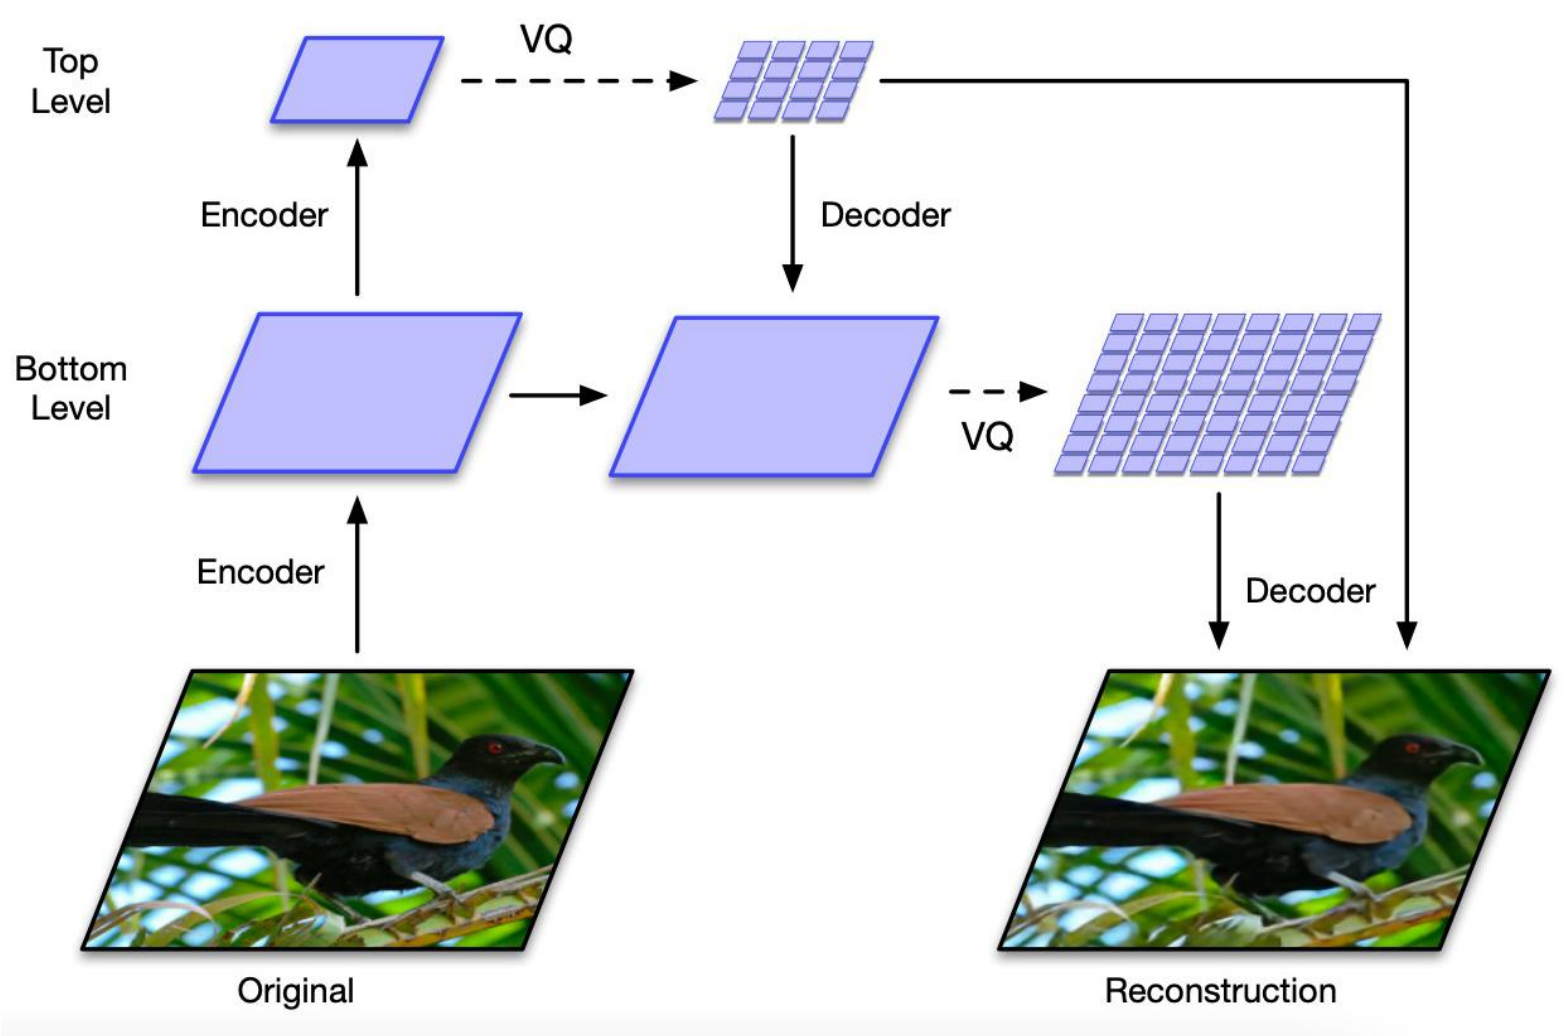
\includegraphics[height=0.9\textheight, width=\textwidth, keepaspectratio]{images/vae/vqvae2.PNG}
     \end{center}
\end{column}
\end{columns}
\end{frame}

\begin{frame}[allowframebreaks]{VQ-VAE Sampling}
\begin{figure}
        \centering
        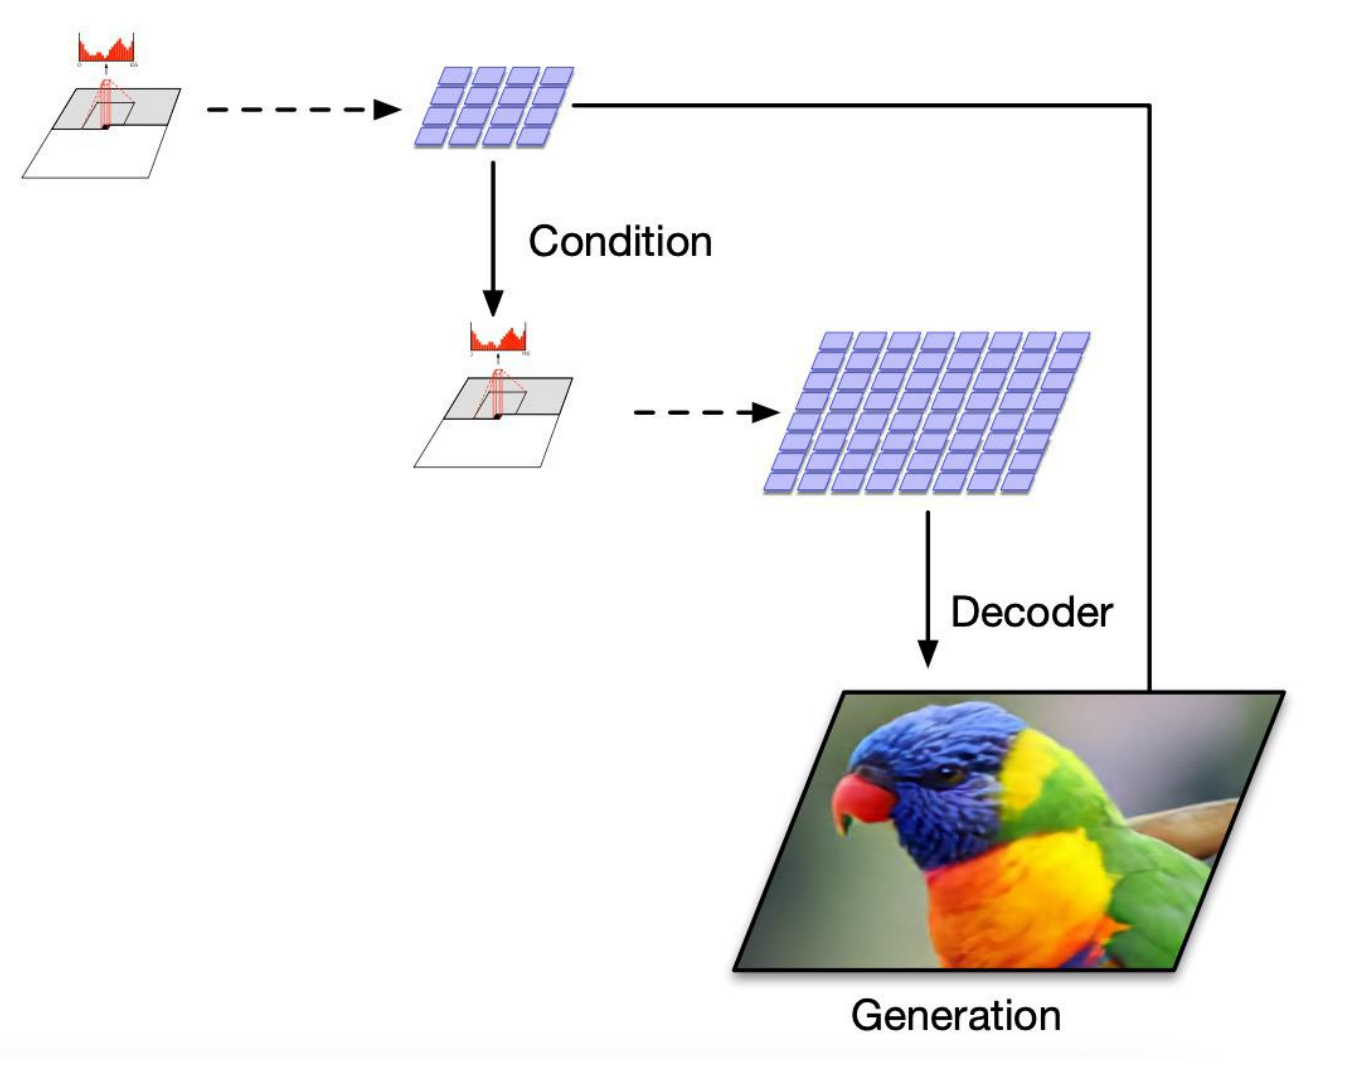
\includegraphics[height=0.9\textheight, width=\textwidth, keepaspectratio]{images/vae/vqvae2_sampling.PNG}
\end{figure}
\end{frame}

\begin{frame}[allowframebreaks]{VQ-VAE ImageNet Samples}
\begin{figure}
        \centering
        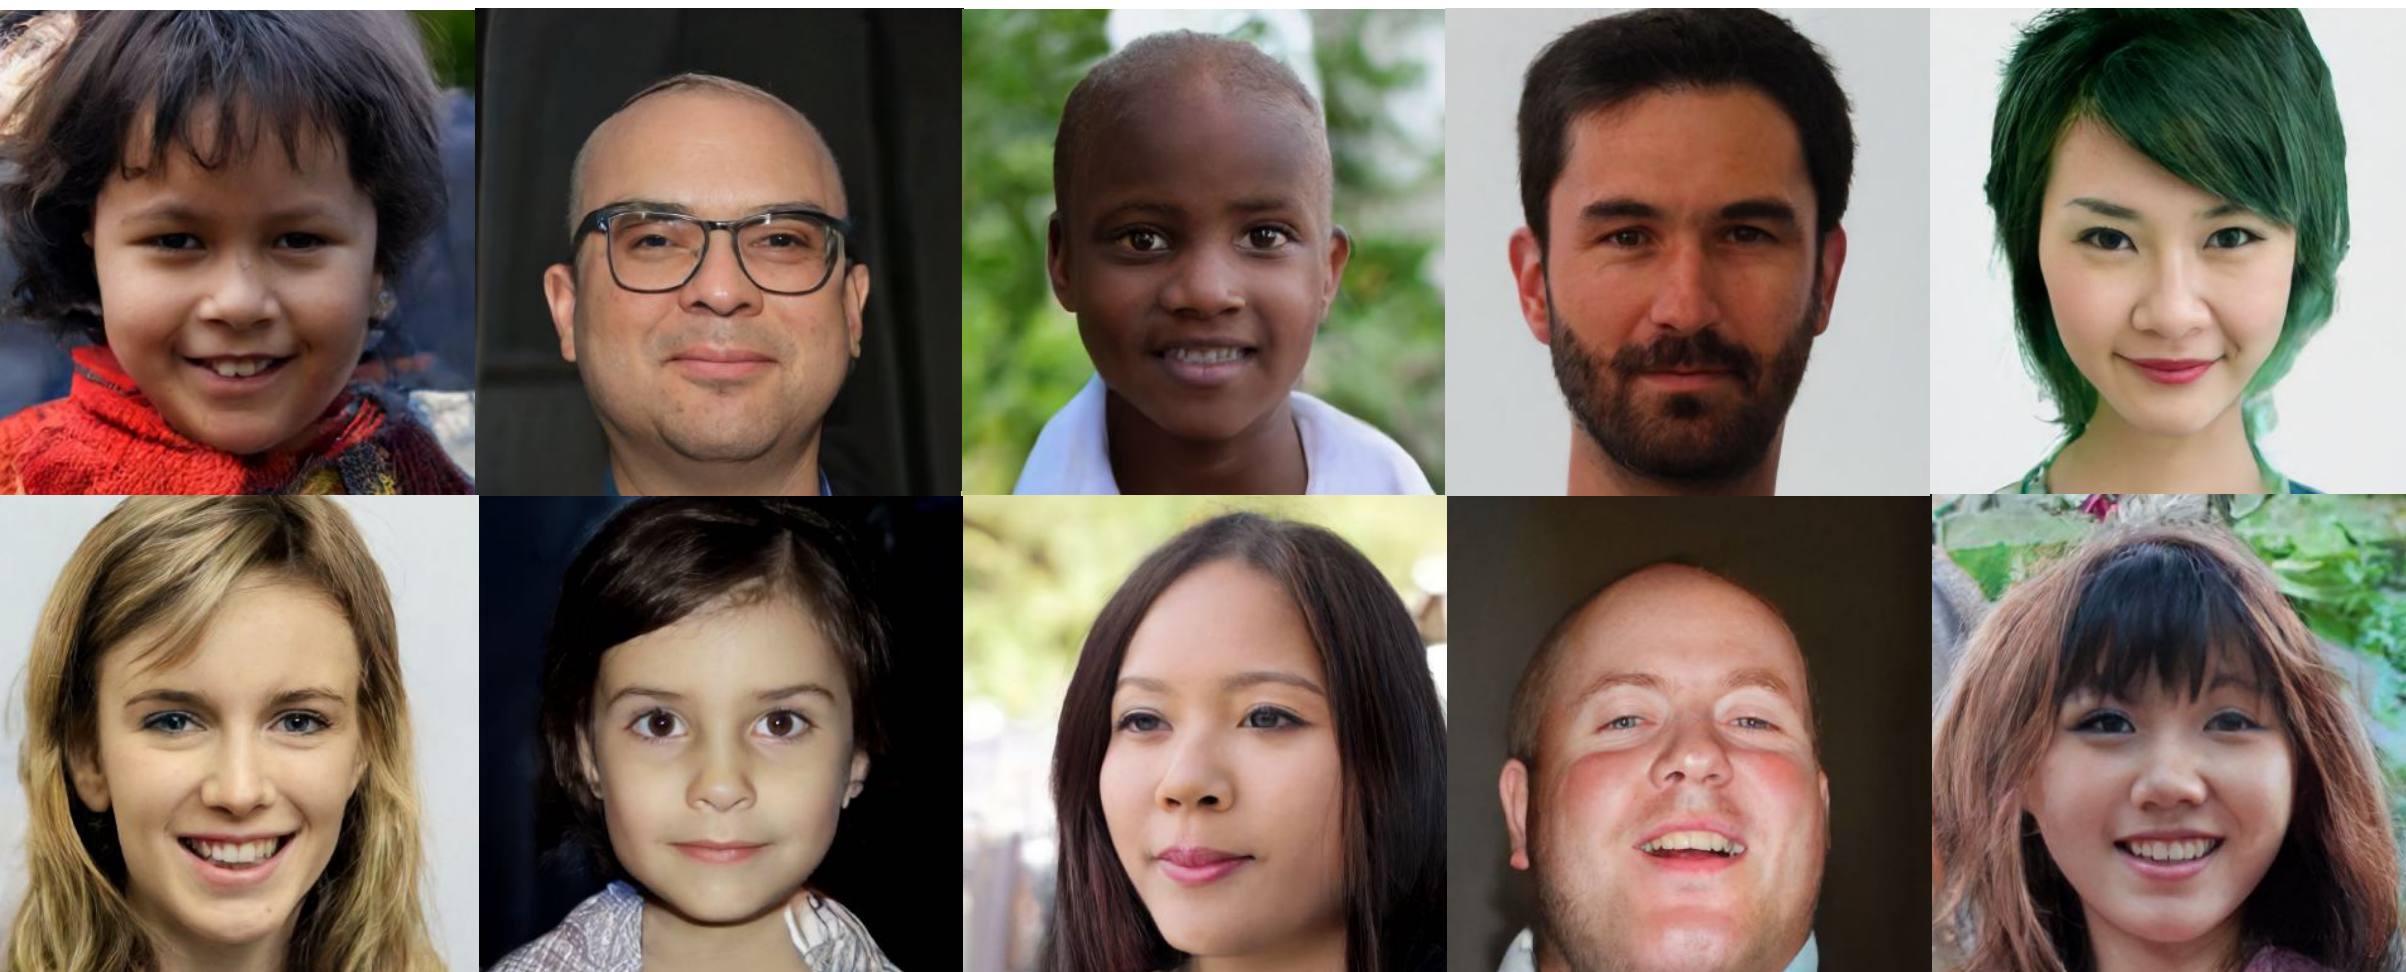
\includegraphics[height=0.9\textheight, width=\textwidth, keepaspectratio]{images/vae/vqvae2_samples.PNG}
\end{figure}
\end{frame}